\section{Introduction}
eBird\cite{DBLP:conf/iaai/KellingGFLWYDG12} is a `citizen science' project that allows for users to report and store bird sightings online. This allows for the crowd-sourcing of bird identification and monitoring, a process that would otherwise require massive amounts of time and effort from researchers. 

While this removes the burden of data collection from experts, it also introduces a number of new problems. In particular, it introduces a higher probability of misidentification (when non-experts attempt to identify birds), and introduces spatial bias, concentrating results around areas of high human population. Thus, data must be sanitized and normalized before it can be used to actually model bird presence. Implemented solutions to these issues are presented in Kelling, et. al~\cite{DBLP:conf/iaai/KellingGFLWYDG12}.

The problem of generating spatially and temporally continuous species distribution from this data is discussed in the `STEM' paper of Fink, et. al~\cite{stem}. We are interested in using the output of this model to explore higher-level questions regarding the movement of migratory birds. In particular, we are interested in inferring an underlying migration network of a given species, given its spatial distribution over time. In our proposed model, nodes in the network represent a contiguous area of the United States, and weighted edges in the network represent the likelihood of bird migration from location to location. 

\begin{figure}[h!]
\centering
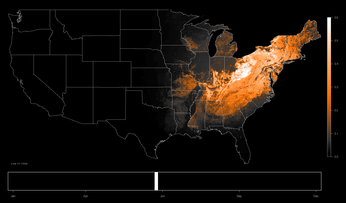
\includegraphics[scale=0.65] {stem}
\caption[Caption for]{Example of STEM output (\url{http://ebird.org/content/ebird/occurrence/})}
\label{fig:00}
\end{figure}
